%& C:\Users\joelv\AppData\Roaming\TikzEdt\TikzEdt\0.2.3.0\temp_header
\begin{document}
\begin{center}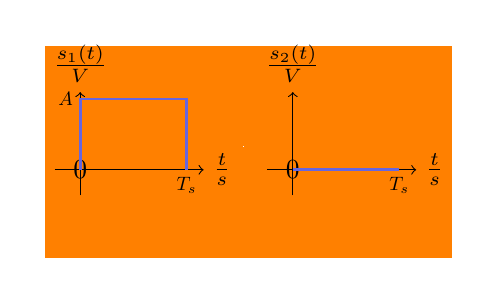
\begin{tikzpicture}[scale=0.9]
\fill[orange]  (-0.5,1.75) rectangle (5.25,-1.25);

\node (null2) at (3,0) {$0$};
\node (startY2) at (3,-0.5) {};
\node (endY2) at (3,1.5) {$\frac{s_2(t)}{V}$};
\node (startX2) at (2.5,0) {};
\node (endX2) at (5,0) {$\frac{t}{s}$};
\draw [->] (startX2) edge (endX2);
\draw [->] (startY2) edge (endY2);

\node (null) at (0,0) {$0$};
\node (startY) at (0,-0.5) {};
\node (endY) at (0,1.5) {$\frac{s_1(t)}{V}$};
\node (startX) at (-0.5,0) {};
\node (endX) at (2,0) {$\frac{t}{s}$};
\draw [->] (startX) edge (endX);
\draw [->] (startY) edge (endY);
\draw[blue!80!black!60, line width=1pt] (0,0) -- (0,1) node[left,black,scale=0.7] {$A$} -- (1.5,1) -- (1.5,0) node[below,black,scale=0.7] {$T_s$};
\draw[blue!80!black!60, line width=1pt] (null2.center) -- (4.5,0) node[below,black,scale=0.7] {$T_s$};

\usetikzlibrary{calc}
\pgftransformreset
\node[inner sep=0pt,outer sep=0pt,minimum size=0pt,line width=0pt,text width=0pt,text height=0pt] at (current bounding box) {};
%add border to avoid cropping by pdflibnet
\foreach \border in {0.1}
  \useasboundingbox (current bounding box.south west)+(-\border,-\border) rectangle (current bounding box.north east)+(\border,\border);
\newwrite\metadatafile
\immediate\openout\metadatafile=\jobname_BB.txt
\path
  let
    \p1=(current bounding box.south west),
    \p2=(current bounding box.north east)
  in
  node[inner sep=0pt,outer sep=0pt,minimum size=0pt,line width=0pt,text width=0pt,text height=0pt,draw=white] at (current bounding box) {
\immediate\write\metadatafile{\p1,\p2}
};
\immediate\closeout\metadatafile
\end{tikzpicture}\end{center}

\end{document}
